\documentclass[14pt]{extbook}
\usepackage{multicol, enumerate, enumitem, hyperref, color, soul, setspace, parskip, fancyhdr} %General Packages
\usepackage{amssymb, amsthm, amsmath, latexsym, units, mathtools} %Math Packages
\everymath{\displaystyle} %All math in Display Style
% Packages with additional options
\usepackage[headsep=0.5cm,headheight=12pt, left=1 in,right= 1 in,top= 1 in,bottom= 1 in]{geometry}
\usepackage[usenames,dvipsnames]{xcolor}
\usepackage{dashrule}  % Package to use the command below to create lines between items
\newcommand{\litem}[1]{\item#1\hspace*{-1cm}\rule{\textwidth}{0.4pt}}
\pagestyle{fancy}
\lhead{Progress Quiz 7}
\chead{}
\rhead{Version ALL}
\lfoot{3510-5252}
\cfoot{}
\rfoot{Summer C 2021}
\begin{document}

\begin{enumerate}
\litem{
Determine the vertical asymptotes and holes in the rational function below.\[ f(x) = \frac{12x^{3} -25 x^{2} -18 x + 40}{16x^{2} +32 x + 15} \]\begin{enumerate}[label=\Alph*.]
\item \( \text{Holes at } x = -0.75 \text{ and } x = -1.25 \text{ with no vertical asymptotes.} \)
\item \( \text{Vertical Asymptote of } x = 0.75 \text{ and hole at } x = -1.25 \)
\item \( \text{Vertical Asymptotes of } x = -0.75 \text{ and } x = -1.25 \text{ with no holes.} \)
\item \( \text{Vertical Asymptote of } x = -0.75 \text{ and hole at } x = -1.25 \)
\item \( \text{Vertical Asymptotes of } x = -0.75 \text{ and } x = 1.333 \text{ with a hole at } x = -1.25 \)

\end{enumerate} }
\litem{
Determine the vertical asymptotes and holes in the rational function below.\[ f(x) = \frac{9x^{3} -12 x^{2} -20 x + 16}{9x^{2} -18 x + 8} \]\begin{enumerate}[label=\Alph*.]
\item \( \text{Vertical Asymptote of } x = 1.333 \text{ and hole at } x = 0.667 \)
\item \( \text{Holes at } x = 1.333 \text{ and } x = 0.667 \text{ with no vertical asymptotes.} \)
\item \( \text{Vertical Asymptotes of } x = 1.333 \text{ and } x = 0.667 \text{ with no holes.} \)
\item \( \text{Vertical Asymptotes of } x = 1.333 \text{ and } x = -1.333 \text{ with a hole at } x = 0.667 \)
\item \( \text{Vertical Asymptote of } x = 1.0 \text{ and hole at } x = 0.667 \)

\end{enumerate} }
\litem{
Which of the following functions \textit{could} be the graph below?
\begin{center}
    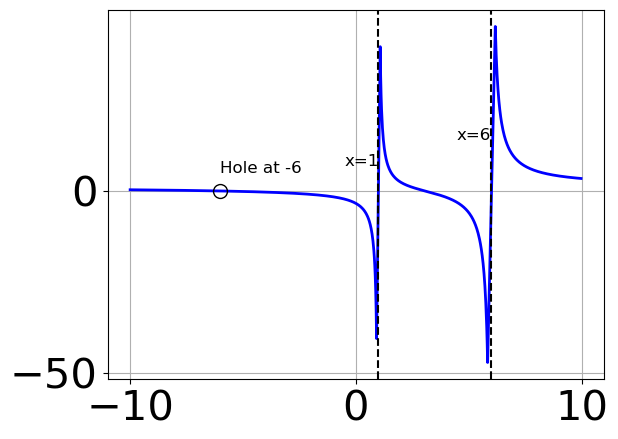
\includegraphics[width=0.5\textwidth]{../Figures/identifyGraphOfRationalFunctionCopyA.png}
\end{center}
\begin{enumerate}[label=\Alph*.]
\item \( f(x)=\frac{x^{3} -37.0 x -84.0}{x^{3} + x^{2} -36.0 x -36.0} \)
\item \( f(x)=\frac{x^{3} -37.0 x + 84.0}{x^{3} -1.0 x^{2} -36.0 x + 36.0} \)
\item \( f(x)=\frac{x^{3} +10.0 x^{2} +3.0 x -126.0}{x^{3} -1.0 x^{2} -36.0 x + 36.0} \)
\item \( f(x)=\frac{x^{3} -10.0 x^{2} +3.0 x + 126.0}{x^{3} + x^{2} -36.0 x -36.0} \)
\item \( \text{None of the above are possible equations for the graph.} \)

\end{enumerate} }
\litem{
Determine the horizontal and/or oblique asymptotes in the rational function below.\[ f(x) = \frac{3x^{2} +16 x + 16}{9x^{3} -36 x^{2} -16 x + 64} \]\begin{enumerate}[label=\Alph*.]
\item \( \text{Oblique Asymptote of } y = 3x -28. \)
\item \( \text{Horizontal Asymptote of } y = 0.333 \text{ and Oblique Asymptote of } y = 3x -28 \)
\item \( \text{Horizontal Asymptote at } y = -4.000 \)
\item \( \text{Horizontal Asymptote of } y = 0 \)
\item \( \text{Horizontal Asymptote of } y = 0.333  \)

\end{enumerate} }
\litem{
Which of the following functions \textit{could} be the graph below?
\begin{center}
    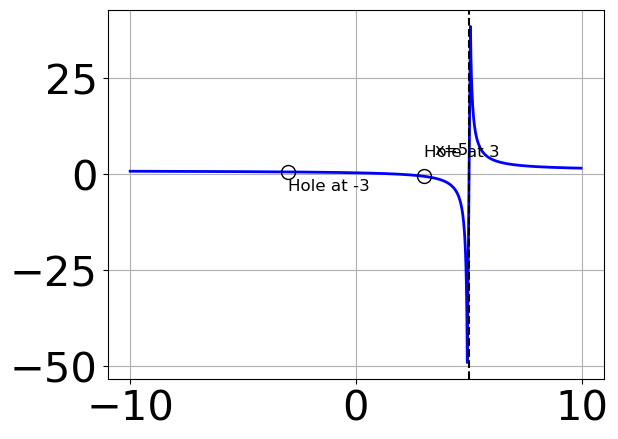
\includegraphics[width=0.5\textwidth]{../Figures/identifyGraphOfRationalFunctionA.png}
\end{center}
\begin{enumerate}[label=\Alph*.]
\item \( f(x)=\frac{x^{3} +7.0 x^{2} +4.0 x -12.0}{x^{3} +5.0 x^{2} -9.0 x -45.0} \)
\item \( f(x)=\frac{x^{3} +2.0 x^{2} -9.0 x -18.0}{x^{3} +5.0 x^{2} -9.0 x -45.0} \)
\item \( f(x)=\frac{x^{3} + x^{2} -16.0 x + 20.0}{x^{3} -5.0 x^{2} -9.0 x + 45.0} \)
\item \( f(x)=\frac{x^{3} -2.0 x^{2} -9.0 x + 18.0}{x^{3} -5.0 x^{2} -9.0 x + 45.0} \)
\item \( \text{None of the above are possible equations for the graph.} \)

\end{enumerate} }
\litem{
Determine the vertical asymptotes and holes in the rational function below.\[ f(x) = \frac{16x^{3} -72 x^{2} +17 x + 60}{8x^{2} -14 x -15} \]\begin{enumerate}[label=\Alph*.]
\item \( \text{Vertical Asymptotes of } x = 2.5 \text{ and } x = -0.75 \text{ with no holes.} \)
\item \( \text{Vertical Asymptotes of } x = 2.5 \text{ and } x = 1.25 \text{ with a hole at } x = -0.75 \)
\item \( \text{Vertical Asymptote of } x = 2.0 \text{ and hole at } x = -0.75 \)
\item \( \text{Vertical Asymptote of } x = 2.5 \text{ and hole at } x = -0.75 \)
\item \( \text{Holes at } x = 2.5 \text{ and } x = -0.75 \text{ with no vertical asymptotes.} \)

\end{enumerate} }
\litem{
Determine the horizontal and/or oblique asymptotes in the rational function below.\[ f(x) = \frac{5x^{2} -29 x + 20}{20x^{3} +49 x^{2} -112 x + 48} \]\begin{enumerate}[label=\Alph*.]
\item \( \text{Oblique Asymptote of } y = 4x + 33. \)
\item \( \text{Horizontal Asymptote of } y = 0 \)
\item \( \text{Horizontal Asymptote of } y = 0.250 \text{ and Oblique Asymptote of } y = 4x + 33 \)
\item \( \text{Horizontal Asymptote of } y = 0.250  \)
\item \( \text{Horizontal Asymptote at } y = 5.000 \)

\end{enumerate} }
\litem{
Determine the vertical asymptotes and holes in the rational function below.\[ f(x) = \frac{8x^{3} -6 x^{2} -45 x + 50}{12x^{2} +5 x -25} \]\begin{enumerate}[label=\Alph*.]
\item \( \text{Vertical Asymptote of } x = -1.667 \text{ and hole at } x = 1.25 \)
\item \( \text{Holes at } x = -1.667 \text{ and } x = 1.25 \text{ with no vertical asymptotes.} \)
\item \( \text{Vertical Asymptotes of } x = -1.667 \text{ and } x = -2.5 \text{ with a hole at } x = 1.25 \)
\item \( \text{Vertical Asymptote of } x = 0.667 \text{ and hole at } x = 1.25 \)
\item \( \text{Vertical Asymptotes of } x = -1.667 \text{ and } x = 1.25 \text{ with no holes.} \)

\end{enumerate} }
\litem{
Determine the horizontal and/or oblique asymptotes in the rational function below.\[ f(x) = \frac{6x^{3} +11 x^{2} -x -6}{2x^{2} +11 x + 12} \]\begin{enumerate}[label=\Alph*.]
\item \( \text{Horizontal Asymptote of } y = -4.0 \text{ and Oblique Asymptote of } y = 3x -11 \)
\item \( \text{Horizontal Asymptote of } y = 3.0 \text{ and Oblique Asymptote of } y = 3x -11 \)
\item \( \text{Horizontal Asymptote at } y = -4.0 \)
\item \( \text{Oblique Asymptote of } y = 3x -11. \)
\item \( \text{Horizontal Asymptote of } y = 3.0  \)

\end{enumerate} }
\litem{
Determine the horizontal and/or oblique asymptotes in the rational function below.\[ f(x) = \frac{6x^{3} -23 x^{2} -16 x + 48}{3x^{2} +8 x -16} \]\begin{enumerate}[label=\Alph*.]
\item \( \text{Horizontal Asymptote of } y = -4.0 \text{ and Oblique Asymptote of } y = 2x -13 \)
\item \( \text{Horizontal Asymptote at } y = -4.0 \)
\item \( \text{Horizontal Asymptote of } y = 2.0  \)
\item \( \text{Horizontal Asymptote of } y = 2.0 \text{ and Oblique Asymptote of } y = 2x -13 \)
\item \( \text{Oblique Asymptote of } y = 2x -13. \)

\end{enumerate} }
\litem{
Determine the vertical asymptotes and holes in the rational function below.\[ f(x) = \frac{9x^{3} +15 x^{2} -74 x + 40}{9x^{2} -9 x -10} \]\begin{enumerate}[label=\Alph*.]
\item \( \text{Vertical Asymptote of } x = 1.0 \text{ and hole at } x = 1.667 \)
\item \( \text{Vertical Asymptotes of } x = -0.667 \text{ and } x = 0.667 \text{ with a hole at } x = 1.667 \)
\item \( \text{Holes at } x = -0.667 \text{ and } x = 1.667 \text{ with no vertical asymptotes.} \)
\item \( \text{Vertical Asymptote of } x = -0.667 \text{ and hole at } x = 1.667 \)
\item \( \text{Vertical Asymptotes of } x = -0.667 \text{ and } x = 1.667 \text{ with no holes.} \)

\end{enumerate} }
\litem{
Determine the vertical asymptotes and holes in the rational function below.\[ f(x) = \frac{6x^{3} +37 x^{2} +75 x + 50}{8x^{2} +30 x + 25} \]\begin{enumerate}[label=\Alph*.]
\item \( \text{Vertical Asymptotes of } x = -1.25 \text{ and } x = -1.667 \text{ with a hole at } x = -2.5 \)
\item \( \text{Vertical Asymptotes of } x = -1.25 \text{ and } x = -2.5 \text{ with no holes.} \)
\item \( \text{Holes at } x = -1.25 \text{ and } x = -2.5 \text{ with no vertical asymptotes.} \)
\item \( \text{Vertical Asymptote of } x = -1.25 \text{ and hole at } x = -2.5 \)
\item \( \text{Vertical Asymptote of } x = 0.75 \text{ and hole at } x = -2.5 \)

\end{enumerate} }
\litem{
Which of the following functions \textit{could} be the graph below?
\begin{center}
    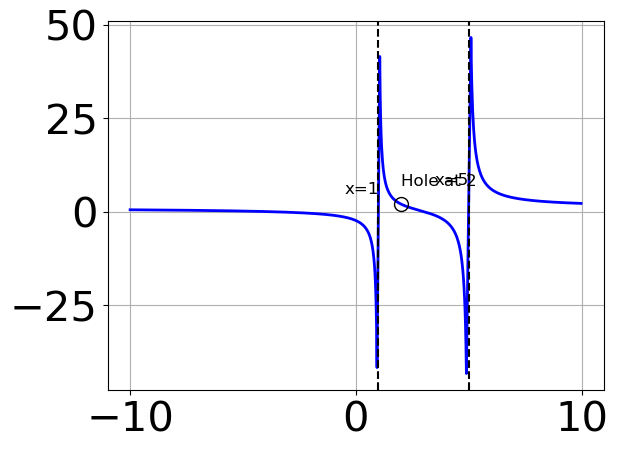
\includegraphics[width=0.5\textwidth]{../Figures/identifyGraphOfRationalFunctionCopyB.png}
\end{center}
\begin{enumerate}[label=\Alph*.]
\item \( f(x)=\frac{x^{3} +5.0 x^{2} -18.0 x -72.0}{x^{3} +8.0 x^{2} +17.0 x + 10.0} \)
\item \( f(x)=\frac{x^{3} -1.0 x^{2} -14.0 x + 24.0}{x^{3} -8.0 x^{2} +17.0 x -10.0} \)
\item \( f(x)=\frac{x^{3} + x^{2} -14.0 x -24.0}{x^{3} +8.0 x^{2} +17.0 x + 10.0} \)
\item \( f(x)=\frac{x^{3} +3.0 x^{2} -10.0 x -24.0}{x^{3} -8.0 x^{2} +17.0 x -10.0} \)
\item \( \text{None of the above are possible equations for the graph.} \)

\end{enumerate} }
\litem{
Determine the horizontal and/or oblique asymptotes in the rational function below.\[ f(x) = \frac{5x^{2} +23 x + 12}{15x^{3} -56 x^{2} +21 x + 36} \]\begin{enumerate}[label=\Alph*.]
\item \( \text{Horizontal Asymptote of } y = 0.333 \text{ and Oblique Asymptote of } y = 3x -25 \)
\item \( \text{Horizontal Asymptote of } y = 0 \)
\item \( \text{Horizontal Asymptote of } y = 0.333  \)
\item \( \text{Oblique Asymptote of } y = 3x -25. \)
\item \( \text{Horizontal Asymptote at } y = -4.000 \)

\end{enumerate} }
\litem{
Which of the following functions \textit{could} be the graph below?
\begin{center}
    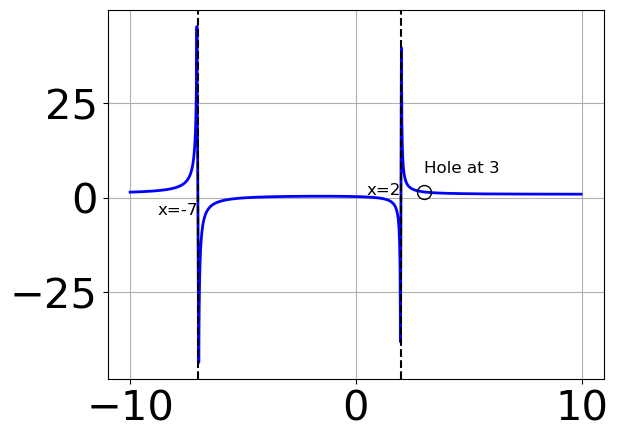
\includegraphics[width=0.5\textwidth]{../Figures/identifyGraphOfRationalFunctionB.png}
\end{center}
\begin{enumerate}[label=\Alph*.]
\item \( f(x)=\frac{x^{3} -1.0 x^{2} -17.0 x -15.0}{x^{3} -2.0 x^{2} -29.0 x -42.0} \)
\item \( f(x)=\frac{x^{3} +8.0 x^{2} +11.0 x -20.0}{x^{3} +2.0 x^{2} -29.0 x + 42.0} \)
\item \( f(x)=\frac{x^{3} +2.0 x^{2} -29.0 x -30.0}{x^{3} -2.0 x^{2} -29.0 x -42.0} \)
\item \( f(x)=\frac{x^{3} + x^{2} -17.0 x + 15.0}{x^{3} +2.0 x^{2} -29.0 x + 42.0} \)
\item \( \text{None of the above are possible equations for the graph.} \)

\end{enumerate} }
\litem{
Determine the vertical asymptotes and holes in the rational function below.\[ f(x) = \frac{4x^{3} -16 x^{2} -25 x + 100}{4x^{2} -4 x -15} \]\begin{enumerate}[label=\Alph*.]
\item \( \text{Vertical Asymptote of } x = 1.0 \text{ and hole at } x = 2.5 \)
\item \( \text{Vertical Asymptotes of } x = -1.5 \text{ and } x = 2.5 \text{ with no holes.} \)
\item \( \text{Holes at } x = -1.5 \text{ and } x = 2.5 \text{ with no vertical asymptotes.} \)
\item \( \text{Vertical Asymptotes of } x = -1.5 \text{ and } x = -2.5 \text{ with a hole at } x = 2.5 \)
\item \( \text{Vertical Asymptote of } x = -1.5 \text{ and hole at } x = 2.5 \)

\end{enumerate} }
\litem{
Determine the horizontal and/or oblique asymptotes in the rational function below.\[ f(x) = \frac{2x^{2} +9 x + 10}{12x^{3} -8 x^{2} -135 x -100} \]\begin{enumerate}[label=\Alph*.]
\item \( \text{Horizontal Asymptote of } y = 0.167  \)
\item \( \text{Horizontal Asymptote at } y = -2.000 \)
\item \( \text{Horizontal Asymptote of } y = 0.167 \text{ and Oblique Asymptote of } y = 6x -31 \)
\item \( \text{Oblique Asymptote of } y = 6x -31. \)
\item \( \text{Horizontal Asymptote of } y = 0 \)

\end{enumerate} }
\litem{
Determine the vertical asymptotes and holes in the rational function below.\[ f(x) = \frac{16x^{3} +16 x^{2} -9 x -9}{8x^{2} -14 x -15} \]\begin{enumerate}[label=\Alph*.]
\item \( \text{Vertical Asymptote of } x = 2.0 \text{ and hole at } x = -0.75 \)
\item \( \text{Vertical Asymptotes of } x = 2.5 \text{ and } x = 0.75 \text{ with a hole at } x = -0.75 \)
\item \( \text{Holes at } x = 2.5 \text{ and } x = -0.75 \text{ with no vertical asymptotes.} \)
\item \( \text{Vertical Asymptote of } x = 2.5 \text{ and hole at } x = -0.75 \)
\item \( \text{Vertical Asymptotes of } x = 2.5 \text{ and } x = -0.75 \text{ with no holes.} \)

\end{enumerate} }
\litem{
Determine the horizontal and/or oblique asymptotes in the rational function below.\[ f(x) = \frac{16x^{3} -16 x^{2} -25 x + 25}{4x^{2} -21 x + 20} \]\begin{enumerate}[label=\Alph*.]
\item \( \text{Horizontal Asymptote of } y = 4.0  \)
\item \( \text{Oblique Asymptote of } y = 4x + 17. \)
\item \( \text{Horizontal Asymptote at } y = 4.0 \)
\item \( \text{Horizontal Asymptote of } y = 4.0 \text{ and Oblique Asymptote of } y = 4x + 17 \)
\item \( \text{Horizontal Asymptote of } y = 4.0 \text{ and Oblique Asymptote of } y = 4x + 17 \)

\end{enumerate} }
\litem{
Determine the horizontal and/or oblique asymptotes in the rational function below.\[ f(x) = \frac{12x^{3} +11 x^{2} -45 x -50}{3x^{2} -7 x -20} \]\begin{enumerate}[label=\Alph*.]
\item \( \text{Horizontal Asymptote at } y = 4.0 \)
\item \( \text{Oblique Asymptote of } y = 4x + 13. \)
\item \( \text{Horizontal Asymptote of } y = 4.0  \)
\item \( \text{Horizontal Asymptote of } y = 4.0 \text{ and Oblique Asymptote of } y = 4x + 13 \)
\item \( \text{Horizontal Asymptote of } y = 4.0 \text{ and Oblique Asymptote of } y = 4x + 13 \)

\end{enumerate} }
\litem{
Determine the vertical asymptotes and holes in the rational function below.\[ f(x) = \frac{6x^{3} -47 x^{2} +112 x -80}{6x^{2} +7 x -20} \]\begin{enumerate}[label=\Alph*.]
\item \( \text{Holes at } x = -2.5 \text{ and } x = 1.333 \text{ with no vertical asymptotes.} \)
\item \( \text{Vertical Asymptote of } x = -2.5 \text{ and hole at } x = 1.333 \)
\item \( \text{Vertical Asymptotes of } x = -2.5 \text{ and } x = 2.5 \text{ with a hole at } x = 1.333 \)
\item \( \text{Vertical Asymptotes of } x = -2.5 \text{ and } x = 1.333 \text{ with no holes.} \)
\item \( \text{Vertical Asymptote of } x = 1.0 \text{ and hole at } x = 1.333 \)

\end{enumerate} }
\litem{
Determine the vertical asymptotes and holes in the rational function below.\[ f(x) = \frac{6x^{3} +11 x^{2} -20 x -25}{9x^{2} -21 x + 10} \]\begin{enumerate}[label=\Alph*.]
\item \( \text{Vertical Asymptote of } x = 0.667 \text{ and hole at } x = 1.667 \)
\item \( \text{Vertical Asymptotes of } x = 0.667 \text{ and } x = 1.667 \text{ with no holes.} \)
\item \( \text{Vertical Asymptote of } x = 0.667 \text{ and hole at } x = 1.667 \)
\item \( \text{Holes at } x = 0.667 \text{ and } x = 1.667 \text{ with no vertical asymptotes.} \)
\item \( \text{Vertical Asymptotes of } x = 0.667 \text{ and } x = -2.5 \text{ with a hole at } x = 1.667 \)

\end{enumerate} }
\litem{
Which of the following functions \textit{could} be the graph below?
\begin{center}
    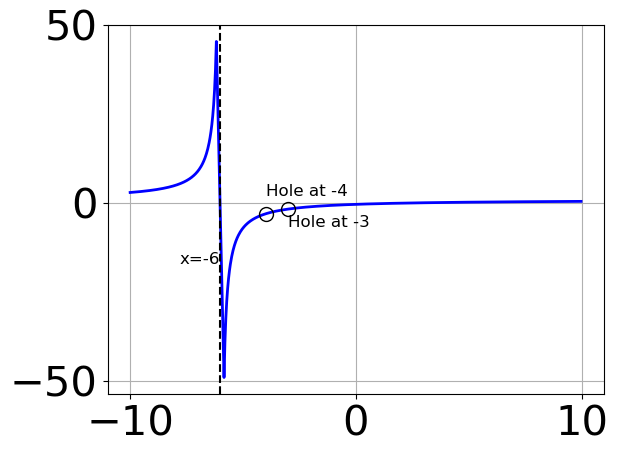
\includegraphics[width=0.5\textwidth]{../Figures/identifyGraphOfRationalFunctionCopyC.png}
\end{center}
\begin{enumerate}[label=\Alph*.]
\item \( f(x)=\frac{x^{3} +5.0 x^{2} -2.0 x -24.0}{x^{3} +13.0 x^{2} +54.0 x + 72.0} \)
\item \( f(x)=\frac{x^{3} -1.0 x^{2} -16.0 x -20.0}{x^{3} -13.0 x^{2} +54.0 x -72.0} \)
\item \( f(x)=\frac{x^{3} -1.0 x^{2} -22.0 x + 40.0}{x^{3} +13.0 x^{2} +54.0 x + 72.0} \)
\item \( f(x)=\frac{x^{3} -5.0 x^{2} -2.0 x + 24.0}{x^{3} -13.0 x^{2} +54.0 x -72.0} \)
\item \( \text{None of the above are possible equations for the graph.} \)

\end{enumerate} }
\litem{
Determine the horizontal and/or oblique asymptotes in the rational function below.\[ f(x) = \frac{20x^{3} -47 x^{2} -54 x + 45}{-20x^{3} +14 x^{2} -18} \]\begin{enumerate}[label=\Alph*.]
\item \( \text{Vertical Asymptote of } y = 3  \)
\item \( \text{Vertical Asymptote of } y = -0.500  \)
\item \( \text{None of the above} \)
\item \( \text{Horizontal Asymptote of } y = 0  \)
\item \( \text{Horizontal Asymptote of } y = -1.000  \)

\end{enumerate} }
\litem{
Which of the following functions \textit{could} be the graph below?
\begin{center}
    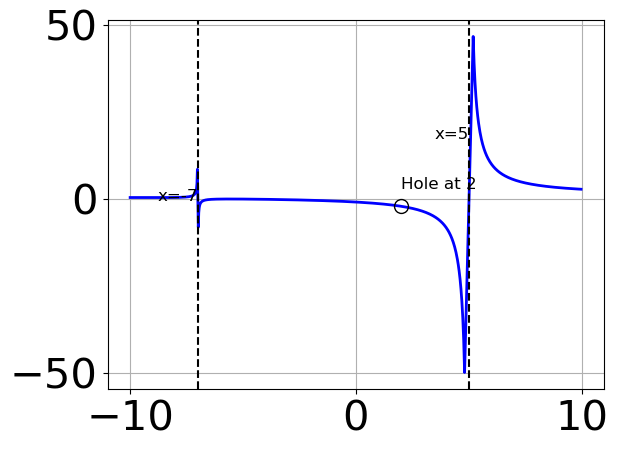
\includegraphics[width=0.5\textwidth]{../Figures/identifyGraphOfRationalFunctionC.png}
\end{center}
\begin{enumerate}[label=\Alph*.]
\item \( f(x)=\frac{x^{3} -5.0 x^{2} -36.0 x + 180.0}{x^{3} -39.0 x -70.0} \)
\item \( f(x)=\frac{x^{3} +13.0 x^{2} +52.0 x + 60.0}{x^{3} -39.0 x + 70.0} \)
\item \( f(x)=\frac{x^{3} +9.0 x^{2} +8.0 x -60.0}{x^{3} -39.0 x + 70.0} \)
\item \( f(x)=\frac{x^{3} -9.0 x^{2} +8.0 x + 60.0}{x^{3} -39.0 x -70.0} \)
\item \( \text{None of the above are possible equations for the graph.} \)

\end{enumerate} }
\litem{
Determine the vertical asymptotes and holes in the rational function below.\[ f(x) = \frac{9x^{3} -9 x^{2} -88 x -80}{9x^{2} +9 x -10} \]\begin{enumerate}[label=\Alph*.]
\item \( \text{Vertical Asymptotes of } x = 0.667 \text{ and } x = -1.333 \text{ with a hole at } x = -1.667 \)
\item \( \text{Vertical Asymptote of } x = 0.667 \text{ and hole at } x = -1.667 \)
\item \( \text{Vertical Asymptote of } x = 1.0 \text{ and hole at } x = -1.667 \)
\item \( \text{Vertical Asymptotes of } x = 0.667 \text{ and } x = -1.667 \text{ with no holes.} \)
\item \( \text{Holes at } x = 0.667 \text{ and } x = -1.667 \text{ with no vertical asymptotes.} \)

\end{enumerate} }
\litem{
Determine the horizontal and/or oblique asymptotes in the rational function below.\[ f(x) = \frac{10x^{3} -13 x^{2} -46 x + 40}{-10x^{3} +46 x^{2} +52 x + 20} \]\begin{enumerate}[label=\Alph*.]
\item \( \text{Vertical Asymptote of } y = -0.400  \)
\item \( \text{Vertical Asymptote of } y = -2  \)
\item \( \text{Horizontal Asymptote of } y = -1.000  \)
\item \( \text{Horizontal Asymptote of } y = 0  \)
\item \( \text{None of the above} \)

\end{enumerate} }
\litem{
Determine the vertical asymptotes and holes in the rational function below.\[ f(x) = \frac{12x^{3} -17 x^{2} -104 x -80}{9x^{2} +6 x -8} \]\begin{enumerate}[label=\Alph*.]
\item \( \text{Vertical Asymptotes of } x = 0.667 \text{ and } x = -1.25 \text{ with a hole at } x = -1.333 \)
\item \( \text{Holes at } x = 0.667 \text{ and } x = -1.333 \text{ with no vertical asymptotes.} \)
\item \( \text{Vertical Asymptotes of } x = 0.667 \text{ and } x = -1.333 \text{ with no holes.} \)
\item \( \text{Vertical Asymptote of } x = 1.333 \text{ and hole at } x = -1.333 \)
\item \( \text{Vertical Asymptote of } x = 0.667 \text{ and hole at } x = -1.333 \)

\end{enumerate} }
\litem{
Determine the horizontal and/or oblique asymptotes in the rational function below.\[ f(x) = \frac{6x^{3} -49 x^{2} +125 x -100}{2x^{2} +3 x -20} \]\begin{enumerate}[label=\Alph*.]
\item \( \text{Horizontal Asymptote at } y = -4.0 \)
\item \( \text{Horizontal Asymptote of } y = 3.0  \)
\item \( \text{Oblique Asymptote of } y = 3x -29. \)
\item \( \text{Horizontal Asymptote of } y = 3.0 \text{ and Oblique Asymptote of } y = 3x -29 \)
\item \( \text{Horizontal Asymptote of } y = -4.0 \text{ and Oblique Asymptote of } y = 3x -29 \)

\end{enumerate} }
\litem{
Determine the horizontal and/or oblique asymptotes in the rational function below.\[ f(x) = \frac{12x^{3} -29 x^{2} +23 x -6}{3x^{2} +10 x -8} \]\begin{enumerate}[label=\Alph*.]
\item \( \text{Horizontal Asymptote of } y = 4.0 \text{ and Oblique Asymptote of } y = 4x -23 \)
\item \( \text{Horizontal Asymptote of } y = -4.0 \text{ and Oblique Asymptote of } y = 4x -23 \)
\item \( \text{Horizontal Asymptote of } y = 4.0  \)
\item \( \text{Horizontal Asymptote at } y = -4.0 \)
\item \( \text{Oblique Asymptote of } y = 4x -23. \)

\end{enumerate} }
\end{enumerate}

\end{document}